\documentclass[8pt]{beamer}
\usepackage[utf8]{inputenc}
\usepackage{xcolor}
\usepackage{colortbl}
\usepackage{epsfig}
% \usepackage{cancel}
\usepackage{ulem}
% \usepackage{threeparttable} % Joao Pela: 
\usepackage{amsmath}
\usepackage{hyperref}
\usepackage{appendixnumberbeamer}
% \usepackage{feynmp}         % For latex produced Feynman Diagrams

% Rule for feynmp diagrams to be considered graphics
% \DeclareGraphicsRule{*}{mps}{*}{}
% 
% % New compile sequence for feynmp
% \makeatletter
% \def\endfmffile{%
%   \fmfcmd{\p@rcent\space the end.^^J%
%           end.^^J%
%           endinput;}%
%   \if@fmfio
%     \immediate\closeout\@outfmf
%   \fi
%   \ifnum\pdfshellescape=\@ne
%     \immediate\write18{mpost \thefmffile}%
%   \fi}
% \makeatother

\usetheme{Madrid}

\author[J. Pela]{João Pela}
\title{Run 2 Trigger Study and VBF QCD samples}
\institute[ICL]{Imperial College London}
\date{2014-04-14}

% The log drawn in the upper right corner.
\logo{\includegraphics[height=0.115\paperheight]{img/Logo_CMSICL.png}}

\begin{document}
\setlength{\unitlength}{1mm}

% ###################################################
\begin{frame}
  \titlepage
\end{frame}

% ###################################################
\begin{frame}{Today's presentation}
 
\begin{block}{Topics}
 
\begin{itemize}
  \item Update on L1 and HLT efficiencies for 13 $TeV$ for the 3 TSG proposed scenarios
  \item Update Comparison between 8 $TeV$ and 13 $TeV$ samples (now including all L1 seeds).
  \item Attempt to use QCD VBF samples to estimate QCD contribution in data
\end{itemize}
 
 
\end{block}

\end{frame}

% ###################################################
\begin{frame}{Samples}

Last time I presented the pythia6 signal samples. For this presentation I have re-run the L1+HLT code (frozen 8E33v2 version) over the POWHEG signal samples. Had to start from GEN-SIM since this is not
possible over AODSIM.

\begin{block}{8 $TeV$ Dataset}

\resizebox{\linewidth}{!}{
\begin{tabular}{|l|c|}
\hline
Sample \\
\hline \hline
/VBF\_HToInvisible\_M-125\_8TeV-powheg-pythia6/Summer12-START53\_V7C-v1/GEN-SIM \\
\hline
\end{tabular}
}

\end{block}

Now both sides (8 TeV and 13 TeV) can be directly compared since they were made using same generator and higgs mass.

\begin{block}{13 $TeV$ Dataset}

\resizebox{\linewidth}{!}{
\begin{tabular}{|l|c|}
\hline
Sample & Events \\
\hline \hline
/VBF\_HToInv\_M-125\_13TeV\_powheg-pythia6/Fall13dr-tsg\_PU20bx25\_POSTLS162\_V2-v1/AODSIM & 484096 \\
/VBF\_HToInv\_M-125\_13TeV\_powheg-pythia6/Fall13dr-tsg\_PU40bx50\_POSTLS162\_V2-v1/AODSIM & 482996 \\
/VBF\_HToInv\_M-125\_13TeV\_powheg-pythia6/Fall13dr-tsg\_PU40bx25\_POSTLS162\_V2-v1/AODSIM & 483696 \\
\hline
\end{tabular}
}

\end{block}
 
\end{frame}

% ###################################################
\begin{frame}{Seeds}

Lets review our HLT paths and their corresponding seeds:

\begin{block}{HLT Paths vs. Seeds}
 
\resizebox{\linewidth}{!}{
\begin{tabular}{|l|l|}
\hline
HLT Path & Seeds \\ 
\hline \hline
HLT\_DiPFJet40PFMETnoMu65MJJ600VBFLeadingJets & L1\_ETM40 \\
HLT\_DiPFJet40PFMETnoMu65MJJ800VBFAllJets     & L1\_ETM40 \\
\hline \hline
HLT\_DiJet20\_MJJ650\_AllJets\_DEta3p5\_HT120\_VBF & L1\_HTT200 OR L1\_HTT175 OR L1\_ETM40 OR L1\_ETM50 \\
HLT\_DiJet30\_MJJ700\_AllJets\_DEta3p5\_VBF        & L1\_HTT200 OR L1\_HTT175 OR L1\_ETM40 OR L1\_ETM50 \\
HLT\_DiJet35\_MJJ650\_AllJets\_DEta3p5\_VBF        & L1\_HTT200 OR L1\_HTT175 OR L1\_HTT150 OR L1\_ETM40 \\
HLT\_DiJet35\_MJJ700\_AllJets\_DEta3p5\_VBF        & L1\_HTT200 OR L1\_HTT175 OR L1\_ETM40 \\
HLT\_DiJet35\_MJJ750\_AllJets\_DEta3p5\_VBF        & L1\_HTT200 OR L1\_HTT175 OR L1\_ETM40 \\
\hline
\end{tabular}
}

\end{block}

Even though we only use L1\_ETM seeded events parked data paths have L1\_HTT seeds too.

\end{frame}

% ###################################################
\begin{frame}{Trigger Efficiencies}

\begin{block}{Efficiencies}
 
\resizebox{\linewidth}{!}{\begin{tabular}{|l||c||c|c|c|}
\hline
& 8 TeV & \multicolumn{3}{|c|}{13 TeV} \\
\hline
Trigger & POWHEG & PU40bx50  & PU20bx25 & PU40bx25 \\
\hline\hline
Events           & $96286$ & $483696$ & $484096$ & $482996$ \\
\hline\hline
\multicolumn{5}{|c|}{Level 1} \\
\hline
L1\_ETM40        & $ 0.4508 \pm 0.0022 $ & $0.4983 \pm 0.0010$ & $0.4808 \pm 0.0010$ & $0.5268 \pm 0.0010 $ \\
L1\_ETM50        & $ 0.3584 \pm 0.0019 $ & $0.4019 \pm 0.0009$ & $0.3893 \pm 0.0009$ & $0.4268 \pm 0.0009 $ \\
L1\_HTT150       & $ 0.0518 \pm 0.0007 $ & $0.2701 \pm 0.0007$ & $0.1467 \pm 0.0006$ & $0.4804 \pm 0.0010 $ \\
L1\_HTT175       & $ 0.0349 \pm 0.0006 $ & $0.1989 \pm 0.0006$ & $0.1025 \pm 0.0005$ & $0.3907 \pm 0.0009 $ \\
L1\_HTT200       & $ 0.0238 \pm 0.0005 $ & $0.1453 \pm 0.0005$ & $0.0718 \pm 0.0004$ & $0.3136 \pm 0.0008 $ \\
\hline\hline         
\multicolumn{5}{|c|}{HLT - Prompt Data} \\
\hline               
HLT\_DiPFJet40\_PFMETnoMu65\_MJJ600VBF\_LeadingJets\_v & $0.0798 \pm 0.0009$ & $0.1092 \pm 0.0005$ & $0.1079 \pm 0.0005$ & $0.1168 \pm 0.0005 $ \\
HLT\_DiPFJet40\_PFMETnoMu65\_MJJ800VBF\_AllJets\_v     & $0.0575 \pm 0.0008$ & $0.0879 \pm 0.0004$ & $0.0850 \pm 0.0004$ & $0.0920 \pm 0.0004 $ \\
\hline\hline
\multicolumn{5}{|c|}{HLT - Parked Data} \\
\hline
HLT\_DiJet35\_MJJ650\_AllJets\_DEta3p5\_VBF\_v         & $0.1125 \pm 0.0011$ & $0.1199 \pm 0.0005$ & $0.1249 \pm 0.0005$ & $0.0793 \pm 0.0004 $ \\
HLT\_DiJet35\_MJJ700\_AllJets\_DEta3p5\_VBF\_v         & $0.1023 \pm 0.0010$ & $0.1100 \pm 0.0005$ & $0.1148 \pm 0.0005$ & $0.0692 \pm 0.0004 $ \\
HLT\_DiJet35\_MJJ750\_AllJets\_DEta3p5\_VBF\_v         & $0.0936 \pm 0.0010$ & $0.1020 \pm 0.0005$ & $0.1062 \pm 0.0005$ & $0.0620 \pm 0.0004 $ \\
HLT\_DiJet20\_MJJ650\_AllJets\_DEta3p5\_HT120\_VBF\_v  & $0.1014 \pm 0.0010$ & $0.1376 \pm 0.0005$ & $0.1498 \pm 0.0006$ & $0.1054 \pm 0.0005 $ \\
HLT\_DiJet30\_MJJ700\_AllJets\_DEta3p5\_VBF\_v         & $0.1125 \pm 0.0011$ & $0.1250 \pm 0.0005$ & $0.1280 \pm 0.0005$ & $0.0776 \pm 0.0004 $ \\
\hline                                                                           
\end{tabular}}

\end{block}

{\tiny
Since last week:
\begin{itemize}
  \item I did found that 2 of the columns were swapped.
  \item Included statistical error on the measurement of efficiency.
  \item Included all L1 triggers that are used to seed out HLT paths.
\end{itemize}

Note:
\begin{itemize}
  \item ETM seeds increase in efficiency slowly with PU.
  \item HTT seeds increase in efficiency with increase of PU (inversely with bunch spacing). Strangely 2X efficiency from PU40bx50 to PU40bx25
  \item All prompt triggers increase efficiency with PU, but parked (with no MET) seem to decrease efficiency.
\end{itemize}
}

\end{frame}

% ###################################################
\begin{frame}{Study of QCD VBF samples to estimate QCD contribution in data}
 
\begin{block}{Method}

\begin{itemize}
  \item Select events that pass BDT just under threshold ($0.1 > BDT_{score} > 0.3$)
  \item Count event on High Delta Phi of data, subtract non QCD bkg and use that number to normalise QCD
  \item Compare plots
\end{itemize}

\end{block}

\begin{columns}
 
\column[t]{0.45\linewidth}
\begin{block}{Without QCD}
 
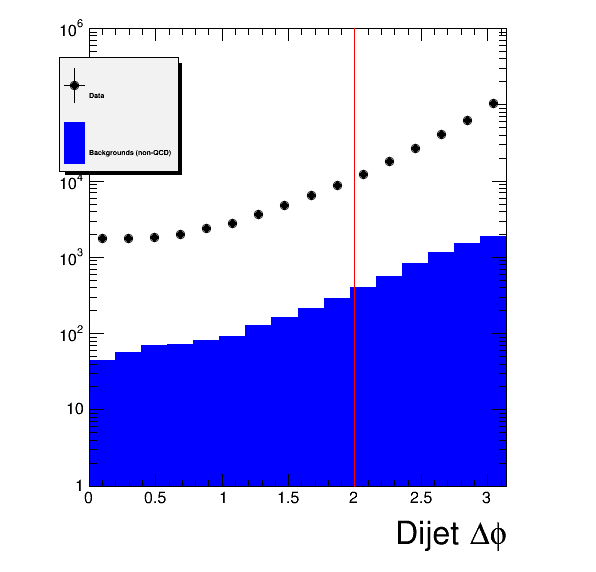
\includegraphics[width=\linewidth]{img/ctrl_dphi.png}
 
\end{block}

\column[t]{0.45\linewidth}
\begin{block}{With QCD}
 
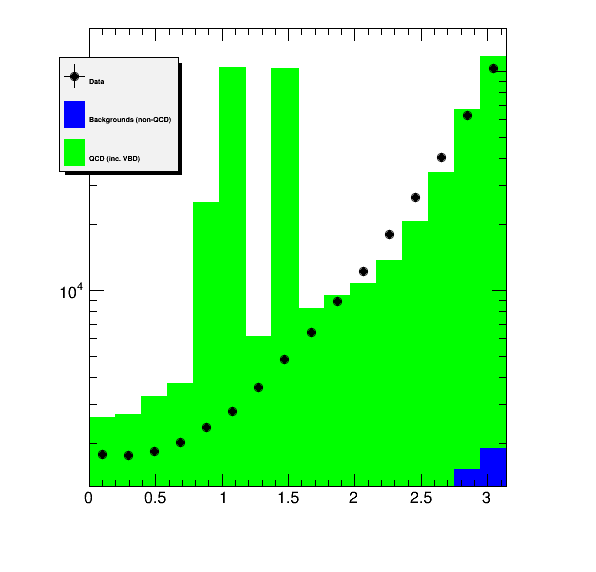
\includegraphics[width=\linewidth]{img/ctrl2_dphi.png}
 
\end{block}

\end{columns}

\end{frame}

% ###################################################
\begin{frame}{Summary and next steps}
 
\begin{block}{Summary:}
 
\begin{itemize}
  \item Trigger study almost finished only HLT candidates study remains. Offline selection analysis would be the next step. 
  \item Looks like there are some significant differences in shape in Delta Phi from VBF QCD to data.
\end{itemize}

\end{block}

\begin{block}{Next Steps:}
 
\begin{itemize}
  \item More plots coming soon.
  \item For discussion.
\end{itemize}
 
\end{block}

\end{frame}


% ###################################################
\appendix
% ###################################################
\begin{frame}
 
\begin{block}

\begin{center}Backup Slides\end{center}

\end{block}

\end{frame}

\end{document}